%%
%% Capítulo 2: Regras gerais de estilo
%%

\mychapter{Fundamentação Teórica}
\label{Cap:Teoria}
Este trabalho envolve a cinemática de um robô móvel,
a implementação de um controlador de estabilizante
que utiliza as leis de controle,
algoritmos de aprendizado de máquina. Portanto esta seção
visa explicar as partes fundamentais destas areas do conhecimento,
que foram utilizada neste trabalho, primeiro abordaremos o problema
da cinemática focando em robôs moveis de acionamento diferencial,
segundo abordaremos o aprendizado de máquina supervisionado
relacionando o tema com a cinemática, terceiro explicaremos o
funcionamento do controlador cinemático de estabilizante criado
por Federico Vieira.

\section{O problema da cinemática de um robô móvel}
Dado um robô de acionamento diferencial, onde as velocidades
angulares das $n$ rodas são: $\phi_0,\phi_1,\phi_2,...,\phi_n$.
Uma cinemática direta $f$ de um robô móvel é a uma função que mapeia as
velocidades
angulares das rodas para a velocidade linear $v$ e velocidade angular $\omega$
do robô, $f(\phi_0,\phi_1,\phi_2,...,\phi_n) \rightarrow v,\omega$. Já
a cinemática inversa $g$, mapeia a velocidade angular e linear do robô para, um
conjunto de velocidades angulares das rodas, $g(v,\omega) \rightarrow  \phi_0,\phi_1,\phi_2,...,\phi_n$.
cinemática é portanto um conjunto de regras que relaciona a velocidade
linear $v$ e angular $\omega$
com as velocidades das rodas $\phi$.

\begin{figure}[H]
    \label{fig:robo:movel:acionamento:diferencial}
    \centering
    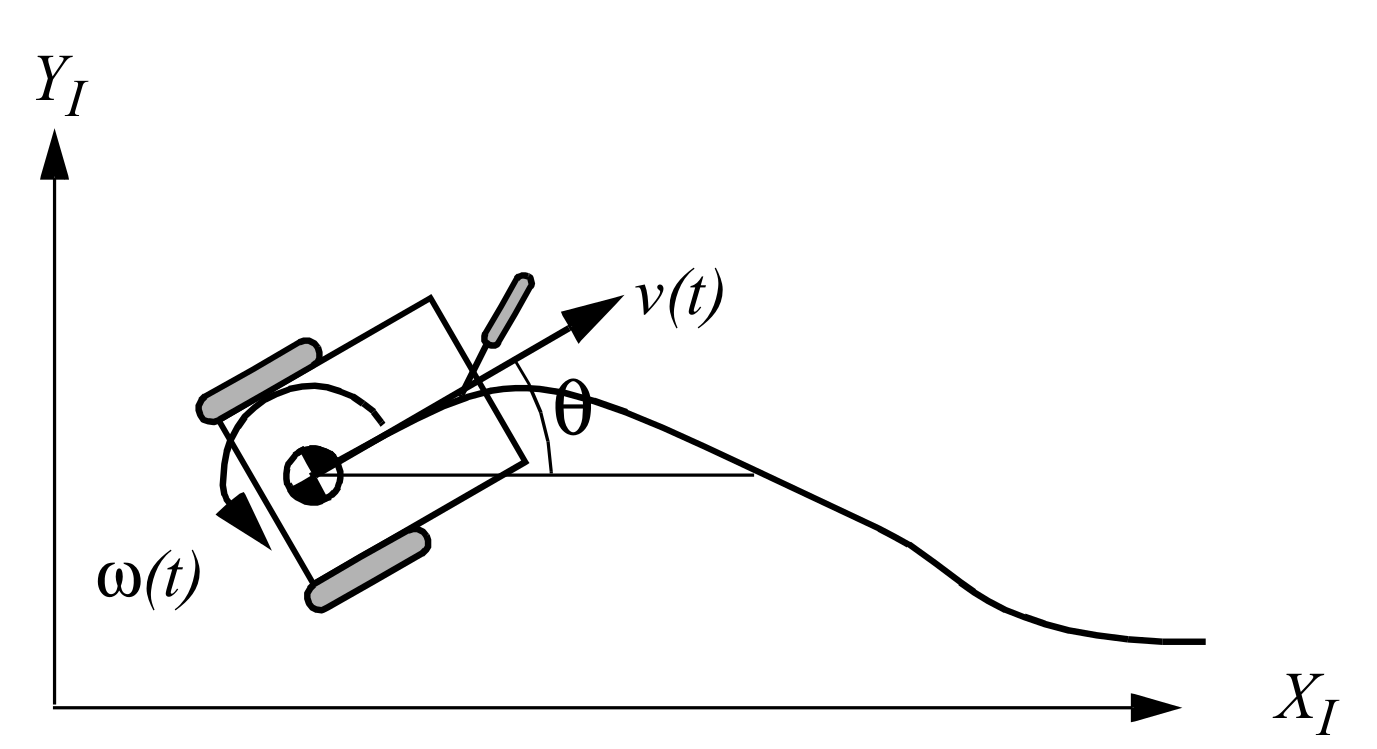
\includegraphics[scale=0.9]{figuras/robo.png}
    \caption{Robô móvel com acionamento diferencial}
\end{figure}

A cinemática de um robô móvel está fortemente relaciona a modelagem
das rodas do robô. Para um robô com duas rodas de acionamento diferencial
como mostrado na figura \ref{fig:robo:movel:acionamento:diferencial}
as equações que regem o movimento dele são:

\[
\begin{bmatrix}
    \sin(\alpha_{1} + \beta_{1}) &  -\cos(\alpha_{1} + \beta_{1}) &  -l_1\cos(\beta_{1})\\
    \sin(\alpha_{2} + \beta_{2}) &  -\cos(\alpha_{2} + \beta_{2}) &  -l_2\cos(\beta_{2})\\
\end{bmatrix}
\begin{bmatrix}
    v_x \\
    v_y \\
    \omega\\
\end{bmatrix}
=
\begin{bmatrix}
    r_0\phi_0 \\
    r_1\phi_1 \\
\end{bmatrix}
\]


\[
\begin{bmatrix}
    \cos(\alpha_{1} + \beta_{1}) &  \sin(\alpha_{1} + \beta_{1}) &  l_n\sin(\beta_{1}) \\
    \cos(\alpha_{2} + \beta_{2}) &  \sin(\alpha_{2} + \beta_{2})  &  l_n\sin(\beta_{2})\\
\end{bmatrix}
\begin{bmatrix}
    v_x \\
    v_y \\
    \omega\\
\end{bmatrix}
=
\begin{bmatrix}
    0 \\
    0 \\
\end{bmatrix}
\]
onde $\alpha$, $\beta$, $l$,$r$ são propriedades das rodas do robô,
$v_x$,$v_y$ são as velocidade lineares ao longo dos eixos x,y.
É importante salientar que os parâmetros das
rodas são extraídos seguindo o referencial do robô $X_r$,$Y_r$ assim como
as velocidades.
\begin{figure}[H]
    \centering
    % 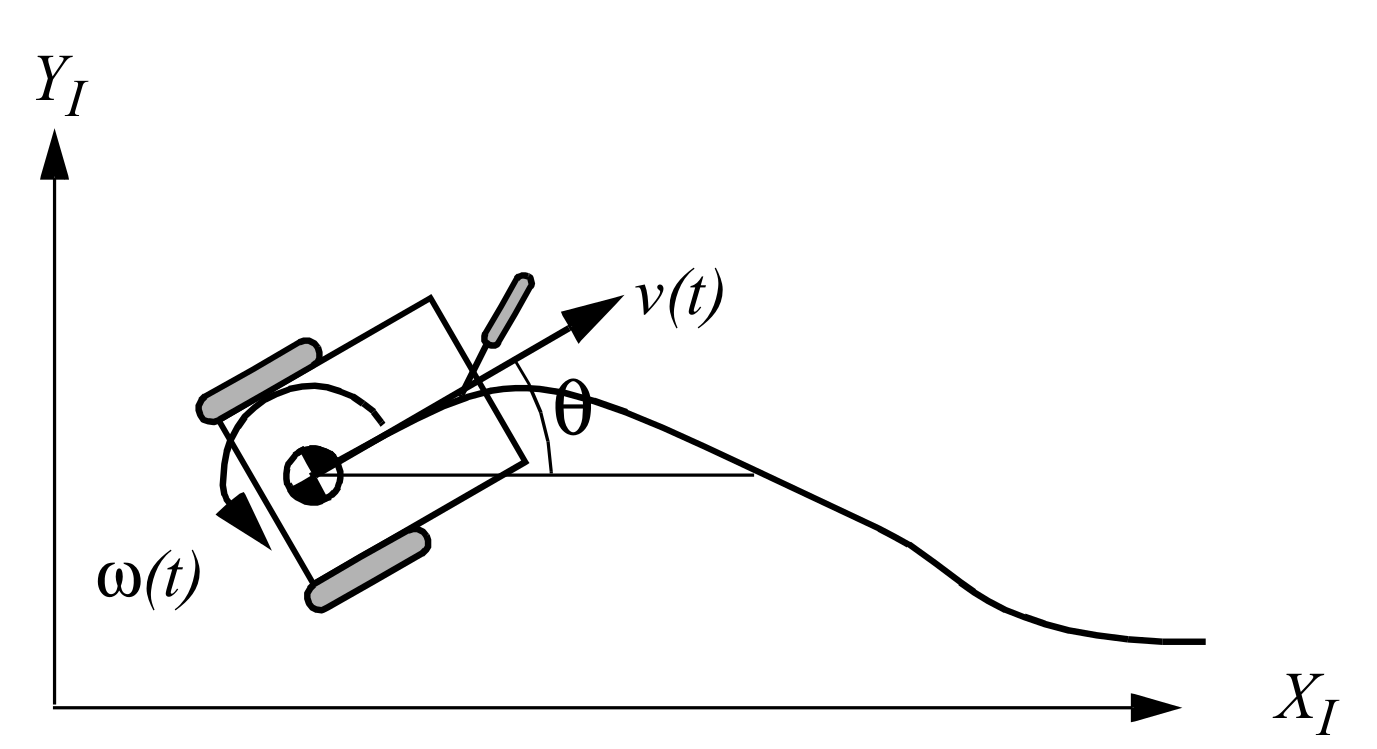
\includegraphics[scale=0.9]{figuras/robo.png}
    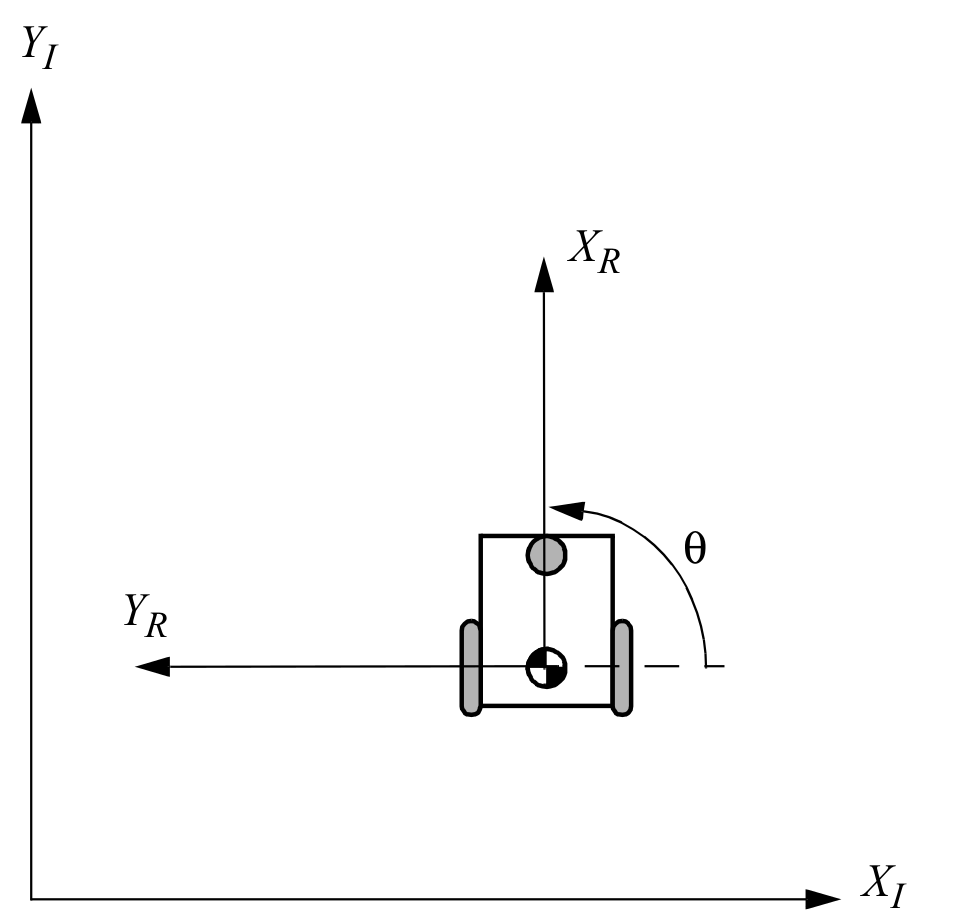
\includegraphics[scale=0.28]{figuras/robo_coordenadas.png}
   
    \[
    \begin{bmatrix}
        v_x \\
        v_y \\
        \omega
    \end{bmatrix}
    =
    \begin{bmatrix}
        cos(\theta)  & sin(\theta) & 0 \\
        -sin(\theta) & cos(\theta) & 0 \\
        0 & 0 & 1 \\
    \end{bmatrix}
    \begin{bmatrix}
        v_{x_I} \\
        v_{y_I} \\
        \omega
    \end{bmatrix}
\]
\caption{Mudança de referencial}
\label{fig:mudanca:referencial}
\end{figure}

Caso a velocidade linear do robô for medida em outro
referencial, é necessário fazer uma rotação do referencial
medido para a orientação $X_r$,$Y_r$. Ná figura \ref{fig:mudanca:referencial}
podemos observar um exemplo de mudança de referencial,
onde $v_{x_I}, v_{y_I}$, são as velocidades no referencial $X_I,Y_I$.

\begin{figure}[H]
    \centering
    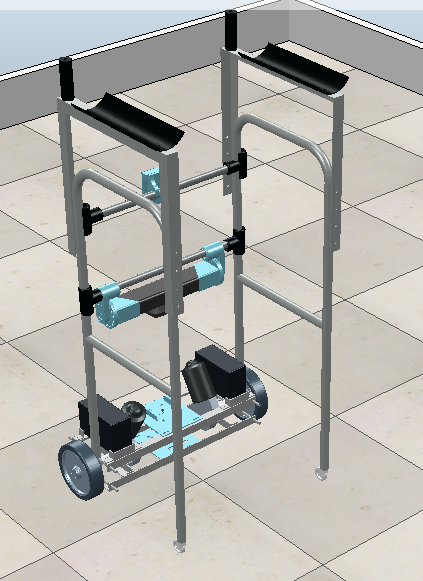
\includegraphics[scale=0.4]{figuras/smart_walker.png}
    \caption{Andador robótico inteligente}
    \label{fig:andador:robotico:inteligente}
\end{figure}


No nosso caso o robô a ser modelado possui quatro rodas, duas delas são
rodas de acionamento diferencial e as outras duas rodas são rodas castores.
Uma imagem do robô pode ser vista na figura \ref{fig:andador:robotico:inteligente}.
Apesar das rodas castores, contribuírem para o movimento, elas não restringem
o movimento, portanto podemos entender o modelo cinemático do nosso robô
como sendo uma transformação linear $W \times X = Y$, onde $X$ é o vetor
de velocidades, e $W$ a matriz de valores constantes obtidas após resolver
as equações.

\begin{figure}[H]
    \[
    \begin{bmatrix}
        W_{11} &  W_{12} & W_{13} \\
        W_{21} &  W_{22} & W_{23} \\
    \end{bmatrix}
    \begin{bmatrix}
        v_x \\
        v_x \\
        \omega \\
    \end{bmatrix}
    =
    \begin{bmatrix}
        \phi_{\text{left}} \\
        \phi_{\text{right}} \\
    \end{bmatrix}
\]
    \caption{Cinemática inversa}
\end{figure}

Um fato muito importante sobre a cinemática do robô de acionamento diferencial
é que resolvendo a cinemática analaticamente vamos perceber que
$\alpha + \beta = 90^{\circ}$ e $\sin(\beta) = 0$, portanto a equação:

\begin{equation}
    v_x\cos(\alpha + \beta)  + v_y\sin(\alpha + \beta) +  \omega l_n\sin(\beta) = 0
\end{equation}

irá se traduzir em:
\begin{equation}
    v_y = 0
\end{equation}
ou seja, segundo a solução analítica não é possível que
o robô translade no eixo y.

\section{Aprendizado de máquina}
Usualmente quando programamos computadores para
resolver determinada tarefa, nós codificamos as regras e
executamos o programa com os dados de entrada e obtemos a resposta.
Esta é a abordagem clássica de se resolver um problema. Uma outra abordagem
é criar sistemas de aprendizado máquina, onde nós possuímos os
dados de entrada, as respontas e queremos que a máquina retorne
para nós quais são as regras que transformam os dados nas respostas
desejadas \cite{chollet2021deep}.

\begin{figure}[H]
    \centering
    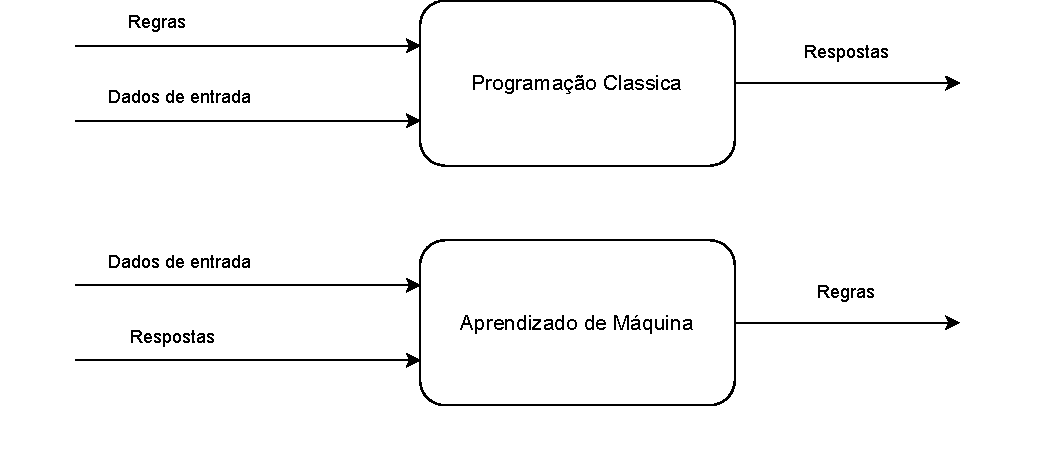
\includegraphics[scale=0.7]{figuras/machine_learning_diagram.pdf}
    \caption{Aprendizado de máquina e Programação clássica}
\end{figure}

Existem três tipos de aprendizado de máquina, aprendizado por reforço,
aprendizado supervisionado e aprendizado não supervisionado.
Aprendizado por reforço é o aprendizado de como mapear situações
para ações de modo que maximize um sinal de recompensa
\cite{sutton2018reinforcement}. Aprendizado supervisionado é o
tipo de aprendizado onde a máquina busca extrair padrões nos conjuntos
de dados de entrada  e do conjunto de dados das respontas de modo que
transforme um dado de entrada na resposta desejada, já aprendizado não
supervisionado também buscar encontrar padrões entre os conjuntos de
dados de entrada e resposta, mas sem ter uma responta correta
\cite{trask2019grokking}. Neste trabalho foi utilizado algoritmos de
aprendizado de máquina supervisionado com objetivo de extrair um modelo de
cinemática inversa do robô andador inteligente.

\begin{figure}[H]
    \centering
    \includegraphics[scale=0.7]{figuras/aprendizado_cinemática_inversa.pdf}
    \caption{Aprendizado de máquina no calculo da cinemática inversa}
\end{figure}

Os algoritmos de aprendizado supervisionado utilizado neste trabalho
foram o Backpropagation e uma variação do algoritmo decida do gradiente, chamada
RMSprop.
Dado uma função $L(M)$, onde $L$ é uma função contínua e derivável,
a decida do gradiente é uma busca que visa encontrar
a melhor matriz $M$ que minimiza uma função $L(M)$, basicamente a
decida do gradiente parte do suposto que existe a sequência
$M_0$, $M_1$, $M_2$, ..., $M_i$, $M_{i+1}$ até $M_k$, onde quando
chegar até $M_k$, o erro $L(M_k)$ será um ponto de mínimo e a transição
entre o $M_{i}$ até $M_{i+1}$, segue a seguinte regra:

\begin{equation}
    M_{i+1} = M_i -\alpha \nabla L(M_i)
\end{equation}

onde $\nabla L(W_i)$ é o gradiente da função erro em relação $M$ aplicado
a $M_i$ e $\alpha$ é um número que varia de 0 até 1,
também conhecido com taxa de aprendizado. Uma variação desse algoritmo
basicamente utilizado é chamado RMSprop, ele se inspira na ideia de momentum
da física  onde  é adicionado uma constante $m$ análoga a massa e uma grandeza
vetorial $v_{\text{vel}}$ análoga a velocidade, criando uma nova equação de decida:

\begin{figure}[H]
    \begin{align*}
        v_{\text{vel}_t} = \alpha v_{\text{vel}_{t-1}} + (1 - \alpha)\nabla L(M_i)^2 \\
        b_t = mb_{t-1} + \frac{\nabla L(M_i)}{\sqrt{v_{\text{vel}_t} + \epsilon}} \\
        M_{i+1} = M_i - b_t
    \end{align*}
    \caption{Equações do RMSprop}
\end{figure}

As variáveis $v_{\text{vel}_t}$ e  $b_t$, são inicializadas como zero, pode acontecer
que  $\sqrt{v_{\text{vel}_t}}$ seja zero ou bem próximo disso então para não ter uma equação
divida por zero é adicionado uma variável $\epsilon =10^{-8}$, deixando o algoritmo numericamente
mais estável. Em contexto de aprendizado supervisionado a função $L$ é uma função erro, que 
através do RMSprop os parâmetros dos modelo são guiados no sentido de minimizar o seu valor.
No entanto não se possui diretamente o gradiente de $L$ em relação aos parâmetros, para isso
é utilizado o  Backpropagation que encontra os gradientes a partir
de pontos $X$ e $Y_{\text{true}}$ coletados. Partindo de  uma definição de um modelo como por exemplo uma
transformação geométrica $Y_{\text{pred}}= A \times X + B$, e uma definição de uma função
erro como: $L=(Y_{\text{true}}- Y_{\text{pred}})^2$ podemos utilizar o algoritmo
Backpropagation para encontrar os gradientes da função $L$ em relação a $A$
e  $B$. Basicamente o Backpropagation executa automaticamente a regra da cadeia
para encontrar os gradientes e com os gradientes podemos executar o RMSprop.

\begin{figure}[H]
    \begin{align*}
        \frac{dL}{dA } = \frac{dL}{dY_{\text{pred}} } \frac{dY_{\text{pred}}}{dA}  \\
        \frac{dL}{dB } = \frac{dL}{dY_{\text{pred}} } \frac{dY_{\text{pred}}}{dB} 
    \end{align*}
    \caption{Regra da cadeia aplicada ao modelo: $Y_{\text{pred}}= A \times X + B$ }
\end{figure}



\section{Controlador estabilizante Vieira}
Controladores cinemáticos ou controladores de movimento, podem ser 
divididos em dois tipos, seguidores de trajetória e estabilizante,
controladores seguidores trajetória recebem como entrada um perfil
de caminho sobre o tempo, a qual o controlador envia sinais de
velocidade linear e angular para o robô de modo que ele siga a
trajetória idealizada, já controladores de estabilizante
eles recebem como entrada um estado atual do robô e o estado desejado
e buscam enviar sinais de velocidade linear e angular com o objetivo
de minimizar o erro entre o estado atual e desejado. Neste trabalho
foi utilizado um controlador de estabilizante criado por Frederico
\cite{vieira2006controle}, o controlador recebe como entrada a posição
$p_c$  no plano x,y , orientação $\theta_c$ atual do robô e uma posição desejada $p_d$
e enviar sinais de velocidade linear $v$ e angular $\omega$ com o
objetivo de estabilizar o robô no ponto desejado.

\begin{figure}[H]
    \centering
    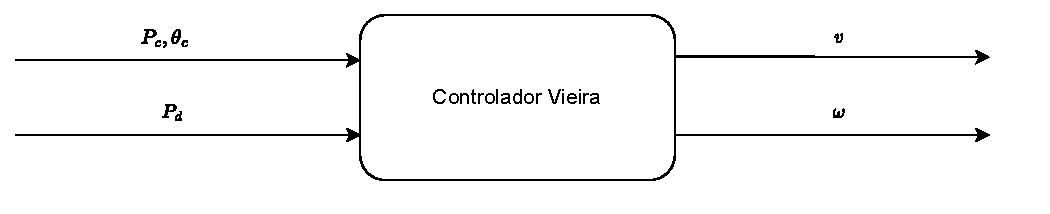
\includegraphics[scale=0.8]{figuras/controlador_viera.pdf}
    \caption{Bloco controlador Vieira}
\end{figure}

Internamente o controlador utiliza  dois controladores proporcionais
integrais derivativos (P.I.D), um controlador é responsável pela velocidade linear $v$
e outro controlador é responsável pela velocidade angular $\omega$. 
Um controlador P.I.D é definido pela a seguinte função de
transferência $C(s)$ no domínio continuo $s$

\begin{equation}
    C(s) = K_p + \frac{K_i}{s} + K_ds
\end{equation}

onde $K_p$,$K_i$,$K_d$ são constantes que podem ser adquiridas ou
através da experimentação ou uma analise matemática \cite{ogataengenharia}. Para gerar sinais
velocidades $v$ e $\omega$,  o controlador Vieira funciona da seguinte
maneira, primeiro é calculado o vetor posição $p_{\text{diff}}$:
\[
    p_{\text{diff}} = p_d - p_c 
\]
segundo são calculadas suas coordenadas polares $l$, $\alpha$:

\[
    l = \sqrt{p_{\text{diff}_x}^2 + p_{\text{diff}_y}^2}
\]
onde $p_{\text{diff}_x}$,$p_{\text{diff}_y}$ são as coordenadas x,y
do vetor $p_{\text{diff}}$.  Terceiro é calculado o angulo $\gamma$:
\[
    \alpha =  \arctan(\frac{ p_{\text{diff}_y}}{p_{\text{diff}_x}}) 
\]

\[
    \gamma =  \alpha - \theta
\]


por fim o controlador P.I.D de velocidade
linear, buscar enviar um sinal $v$ que faça tender o valor $l \cos(\gamma)$
a zero e o controlador de velocidade angular busca enviar um sinal $\omega$
para  tender o valor de $\gamma$ a zero. Perceba que quando o valor de $\gamma$
tende a zero, a velocidade linear vai tender a reduzir apenas
distância $l$. Como o modelo cinemático do robô espera receber como entrada
um vetor de velocidade linear em coordenadas cartesianas então é preciso
transformar de volta a velocidade $v$ 

\[
    \begin{bmatrix}
        v_x \\
        v_y \\
    \end{bmatrix}
    =
    \begin{bmatrix}
        v\cos(\theta) \\
        v\sin(\theta) \\
    \end{bmatrix}
\]
onde, $v_x$, $v_y$ são as velocidade lineares em coordenadas cartesianas.